To implement The data driven machine learning technique detect suspicious companies to prevent trade credit fraud, below system design was used. The design is broadly broken down into main three components. These are Data Mining, Model Configuration, and Model selection. In below sections each of the components are described. 


\begin{figure}[h]
    \centering
    \begin{tikzpicture}[font=\small,thick]

        % Start block
        \node[draw,
            rounded rectangle,
            minimum width=1.5cm,
            minimum height=1cm] (block1) {START};
        
            
        % Voltage and Current Measurement
        \node[draw,
            trapezium, 
            trapezium left angle = 65,
            trapezium right angle = 115,
            trapezium stretches,
            below=of block1,
            minimum width=2.5cm,
            minimum height=1cm
        ] (block2) {Data mining};
        
        \node[draw,
            align=center,
            below=of block2,
            minimum width=2.5cm,
            minimum height=1cm
        ] (block3) {Building Model};
        
        
        \node[draw,
            diamond,
            below=of block3,
            minimum width=2.5cm,
            inner sep=0] (block4) {Model Selection};
        
       
        % Arrows
        \draw[-latex] (block1) edge (block2)
            (block2) edge (block3)
            (block3) edge (block4);
        
        \end{tikzpicture}
    \caption{Application Design}
    \label{fig:my_label}
\end{figure}
\mytodo{update the flowchart}

\subsection{Data Mining}
The most important aspect to train a complex system like is to feed adequate data set, so that model can perform well. However, the information required for preparing dataset is not readily available. In below sub sections the steps of Data mining is described. 
\subsubsection{Source Identification}\hspace*{\fill} \\
The subject matter experts are the first point of contact to identify the source to identify the suspicious companies. It is important to understand how traditionally the auditors, credit under taking team analyse the data and identify the key indicators. In the end of the day fraudulent transaction or activity is a human behaviour, hence the experts in this field look for particular patterns and indicators to identify the suspicious entity. The pattern in the financial transaction and general activities of the company are monitored to identify the patters. Below repetitive steps are taken to identify each key indicators.

\begin{enumerate}
    \item Make a comprehensive list of all possible indicators by taking notes from different subject matter experts. 
    \item Identify if there is any human biases on selected indicators  
    \item Determine if the identified variable is a binary (flag) or continues variable. 
    \item Identify the source of the data, i.e. internal source (financial statements, company profile) or external source. 
\end{enumerate}
\subsubsection{Data Extraction}\hspace*{\fill} \\
The next activity to prepare the training data set is to extract data from historical company information. Based on the selected key indicators the combines sources are identified. For the current problem its been found that majority of the information are coming from company financial information kept is a Oracle database and historical company reports which are kept in Extensible Markup Language (xml) format. For data extraction step all the indicators for past 10 years have been taken from these sources. The extracted information is kept in MongoDB server where the information of each companies are kept. The financial information are fetched from existing oracle DB, however the vital company information are extracted from the XML and kept in a JSON \mytodo{cite} format for further uses. 

\mytodo{Flow diagram needs to be added}

\subsubsection{Feature Engineering}\hspace*{\fill} \\
After the features extraction feature engineering is done to generate features based on the identified indicators. The engineered features are based on the financial information, company activities and recombination of the information. Due to sensitivity of the data, the details of the features are not mentioned. However below are the general overview of the feature engineering

\begin{itemize}
    \item \textbf{Financial:} The historical and recent financial information of each company have been collected. This data shows the trend and pattern of the company over last 10 years. During features extraction the anomalies are flagged and converted into a binary variable. There are lots of floating points information like yearly profit are kept as continues variable. 
    
    \item \textbf{Non Financial:} The non financial features are mainly based on the behavioural aspect of personal and the company. As the behavioural information is not easily transferable to features, the important activities and characteristics are marked and binary or continues variable. Information like trade sector, abnormal changes of company, vital dates, recent suspicious transactions etc. are engineered as features.
    
    \item \textbf{Combination:} It was noticed that some of the useful additional features can be mined using the combination method. In a combination method new feature can be created combining two or more financial or non financial features by using logical or mathematical process. For example a new marker can be created to find the ratio of number of employees and overall financial turnover of the company. 
\end{itemize}

below pseudo code structure [Algorithm :\ref{alg:feature}]is used to engineer features from extracted data . 

\begin{algorithm}
\caption{Feature Engineering}
\label{alg:feature}
\SetKwProg{feature}{Function \emph{feature}}{}{end}

    \feature{(Company Object)}{
        \textbf{Input:}{ company information in JSON formal} \\
        \textbf{Output:}{ feature value (int - flag, float for continues variable}
  
        \State {$feature\_counter \gets 0$ \CommentSty{Initialise the counter}} \\
        
        \If{ $report\_date$ is available}{
              $important\_date$ = $report\_date$\;
          }
        \Else{}{\Return $feature\_counter$}
         
        \State {$json\_expression$ \= parse JSON to get feature information} \\
        \State{$list \gets$ value from $json\_expression$ }\\
       \\
        \ForAll{child $c$ in list}{
            \If{$important\_date \leq child['date']$ }{
                    $feature\_counter$ ++
                }
             
        }
        \Return $feature\_counter$\\
    }
\end{algorithm}


\subsubsection{Exploratory data analysis}\hspace*{\fill} \\

From the feature extraction and feature engineering stage we get the full data set. To prepare the dataset total last 10 years of data for all companies (having \mytodo{cla} date) are selected. Due to time complexity for data extraction and keep to understand only recent trend last 10 years data is considered. In the data set we can see the there are total 30 columns, however the number of features are 27. The total number of features are 48,549. Among this data only 1358 are marked fraudulent or suspicious company. The actual data is around 100k during this period. However to keep the data mining time low, the dataset size kept to 48,549. From the paper on SMOTE \cite{}, we have seen the under sampling with SMOTE performs re lately well. So theoretically the performance will still get improvement.
\begin{itemize}
    \item Total number of columns: 30
    \item Number of company entries: 48,539
    \item Target label: Fraudulent
    \item Total Features: 27
    \item Total Fraudulent / suspicious: 1358
\end{itemize}

From the initial assessment we can see the that classes are very imbalanced. In the dataset there is only 1358 fraudulent cases out of 48,549 ones. That means only 2.8\% of companies are fraudulent or specious. 

\begin{figure}[H]
    \centering
    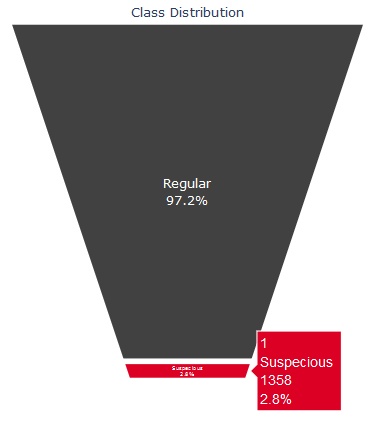
\includegraphics[width=.8\linewidth]{figures/class_imbalance.png}
    \caption{Class Distribution}
    \label{fig:class distribution}
\end{figure}

The complexity to build a model to detect a huge obstacle. In the features \ref{fig:Dimension reduction}
\begin{figure}[H]
    \centering
    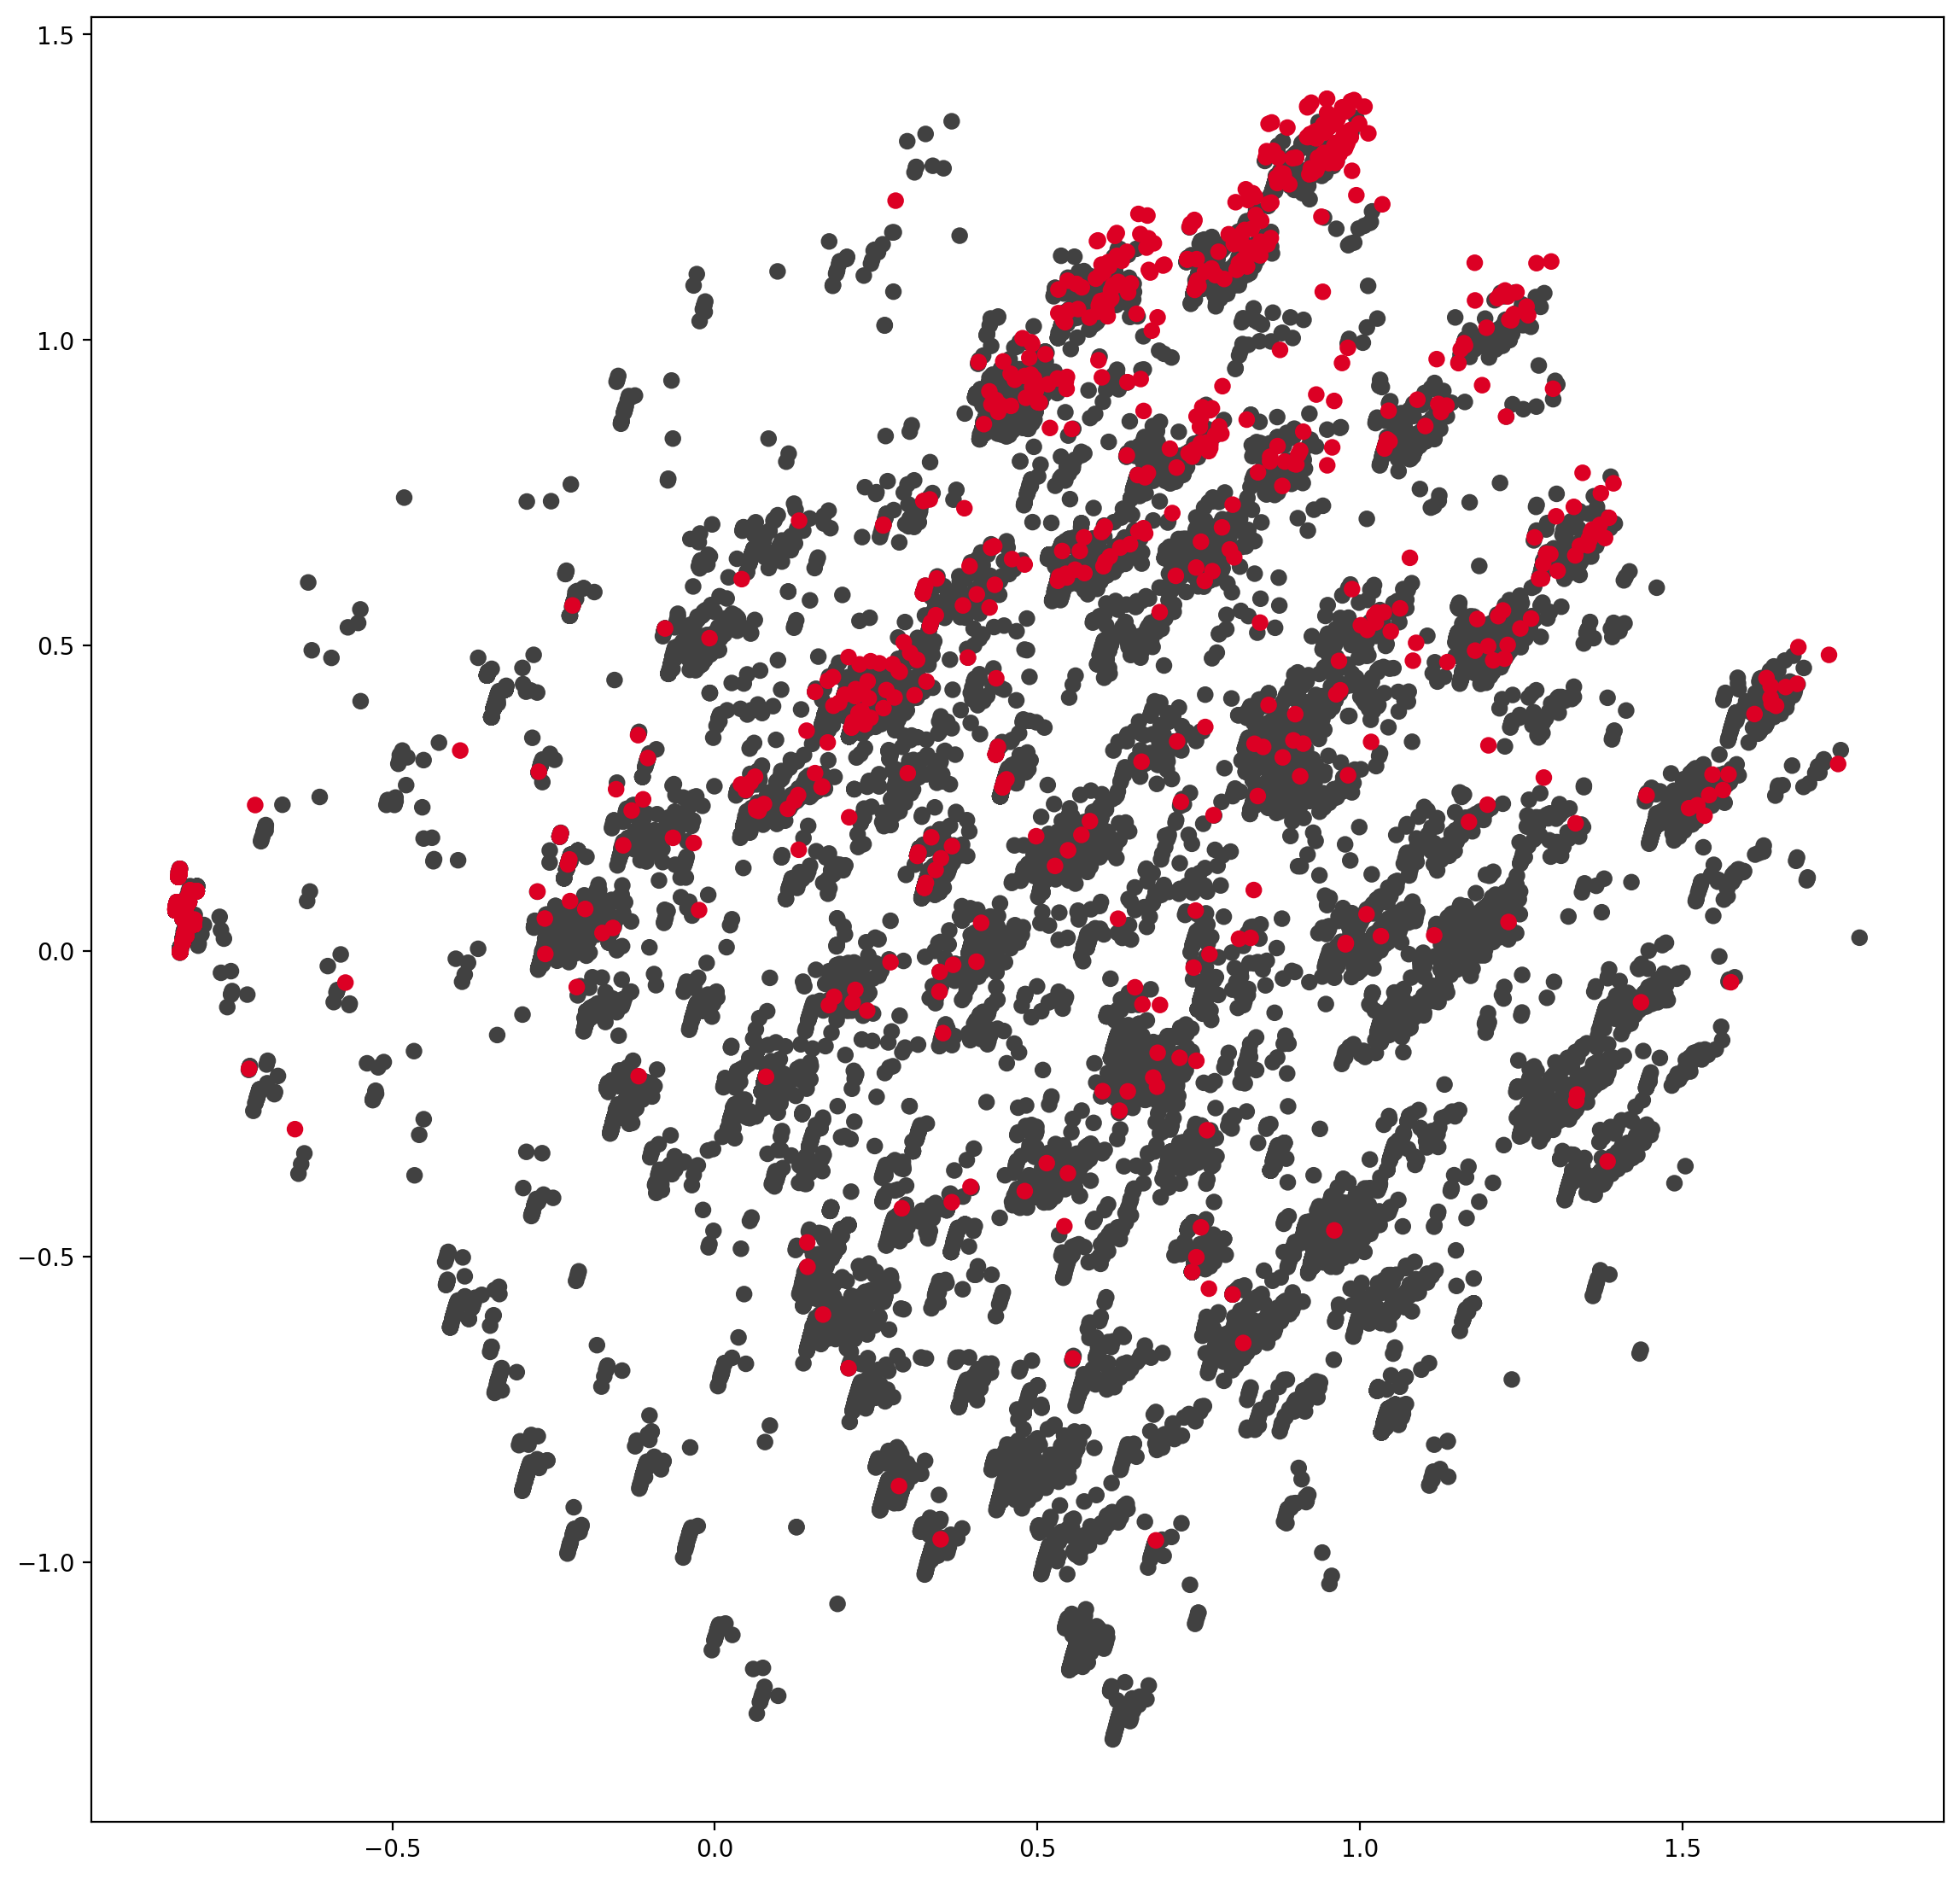
\includegraphics[width=\linewidth]{figures/pca_2d.png}
    \caption{Dimension reduction}
    \label{fig:Dimension reduction}
\end{figure}
The proportion of the fraudulent cases is shown in figure \ref{fig:feature proportion}. 
\begin{figure}[H]
    \centering
    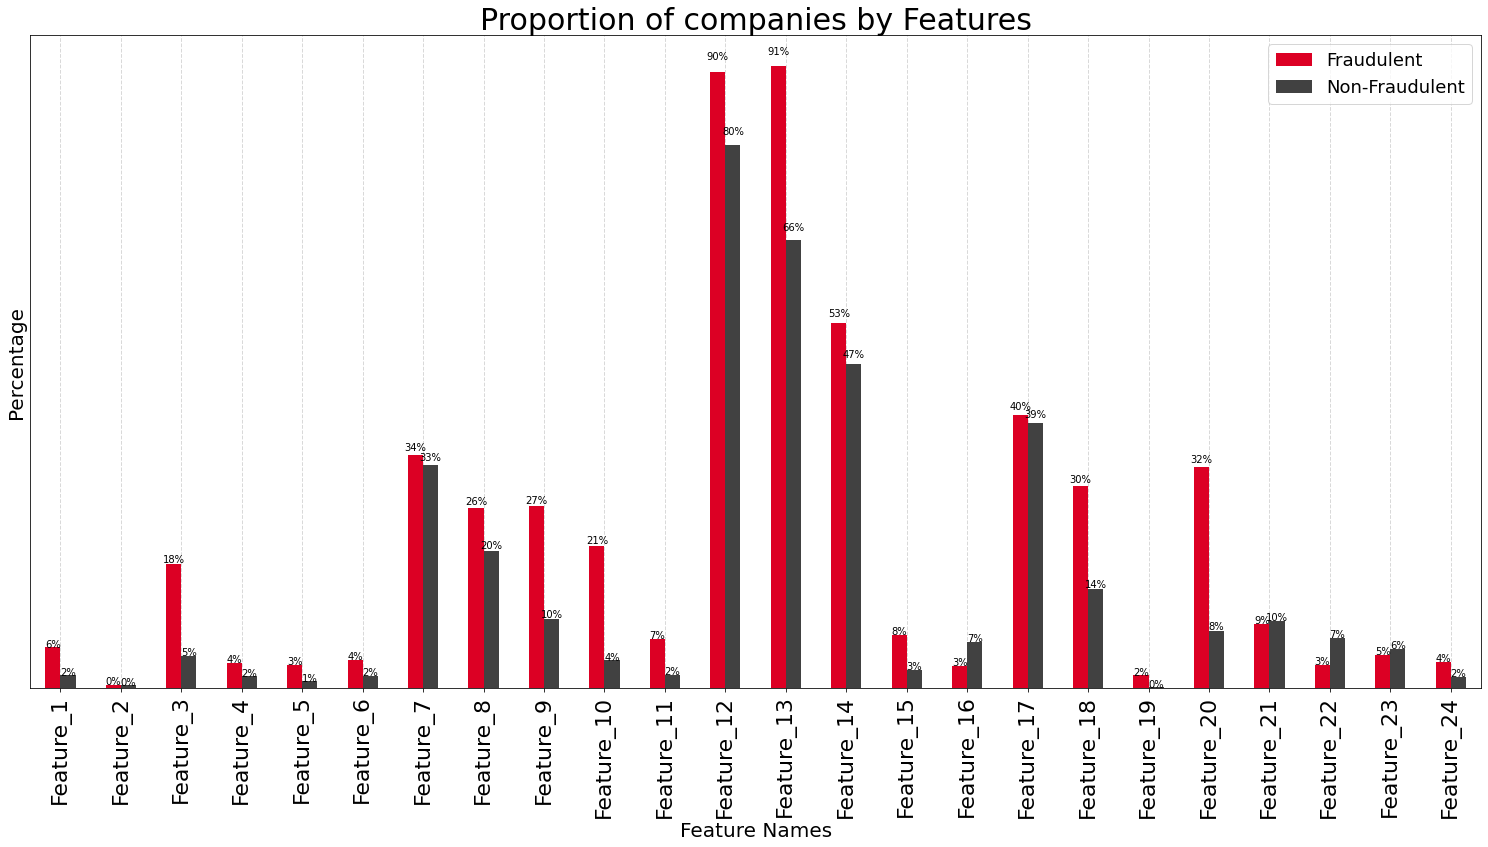
\includegraphics[width=\linewidth]{figures/feature_proportion.png}
    \caption{Proportion of binary features}
    \label{fig:feature proportion}
\end{figure}

\begin{figure}[H]
    \centering
    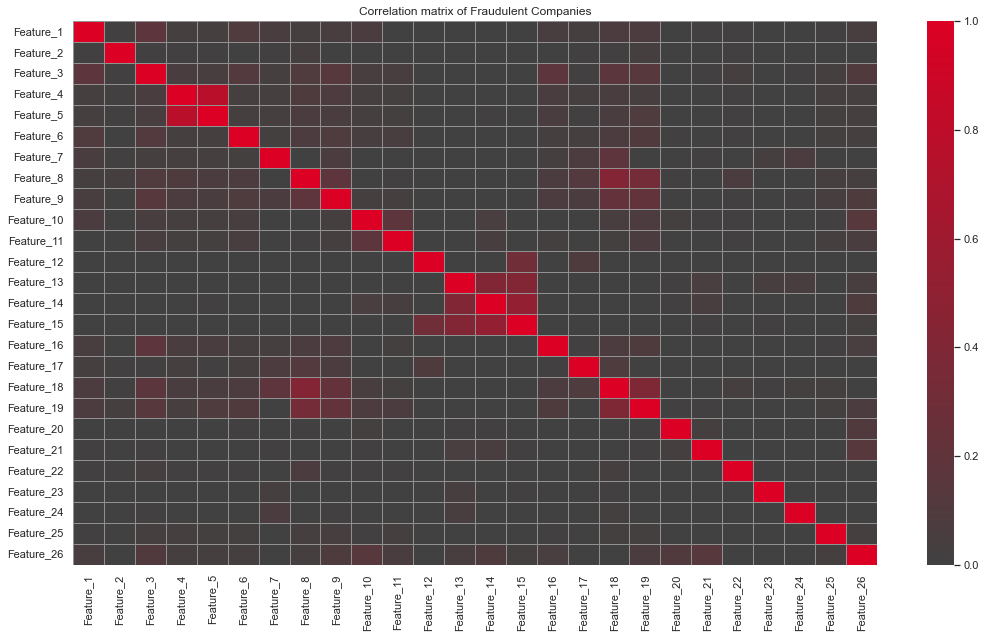
\includegraphics[width=\linewidth]{figures/corr.png}
    \caption{Correlation Matrix}
    \label{fig:corr}
\end{figure}

\subsubsection{Dataset Finalisation}\hspace*{\fill} \\
Finally the dataset has been segmented into train and test sets. From the
\begin{itemize}
    \item \textbf{Train and test split:}
    \item \textbf{Data Pre-processing:}
    \item \textbf{Handle class Imbalance:}
\end{itemize}

\subsection{Model configuration}

\subsubsection{Random Forest}\hspace*{\fill} \\
Random forest algorithm generally performs better compare with other classification algorithms for imbalanced dataset \cite{Valecha2018PredictionOC}. In random forest model classifier ensemble different trees and final prediction happens by voting and selecting the majority decision. 

\begin{enumerate}
    \item Randomly select N number of Features
    \item Train a Decision Tree with selected features
    \item Select the target number of tress and repeat first two steps 
    \item Each tree predicts the class for new entry
    \item The final class prediction done by majority vote. 
\end{enumerate}

In our random forest,we set tree number to 200. We also use grid search method to set some ratio of the class weights and other related parameters to select the most suitable one with the highest accuracy. For example,the class weight selection process is shown in Fig.2. As the figure shows, when our weights equals to the ratio of 1:1 and 1:2, our accuracy perform best. Therefore, we set the class weight as 1:1 in the experiment.Also there are some other parameters we will not enumerate here but the process are the same. \mytodo{text needs to be updated}



\textbf{Hyper-parameter tuning:}
Random Forest classifiers comes with crucial parameters which needs to be tuned to get the best model. Below parameters are used in a random grid search method to do hyper parameter tuning for the random forest estimator. The options for each estimators are shown in the table: ~\ref{tab:RF_param}.
\begin{itemize}
    \item n\_estimator: Number of trees in random forest
    \item max\_features: Number of features to consider at every split
    \item max\_depth: Maximum number of levels in tree
    \item min\_samples\_split: Minimum number of samples required to split a node
    \item min\_sample\_leaf: Minimum number of samples required at each leaf node
    \item bootstrap: Method of selecting samples for training each tree
\end{itemize}

\begin{table}[h]
    \begin{tabular}{llll}
    Parameter           & Options         & No of options \\
    n\_estimator        & 200 to 2000     & 100           \\
    max\_features       & Auto, sqrt      & 2             \\
    max\_depth          & None, 10 to 110 & 12            \\
    min\_samples\_split & 2,5,10          & 3              \\
    min\_samples\_leaf  & 1,2,4           & 3              \\
    bootstrap           & True, False     & 2              \\
    \end{tabular}
    \caption{Hyper-parameter settings for Random Forest}
    \label{tab:RF_param}
\end{table}


\subsubsection{XDBoost}\hspace*{\fill} \\
\mytodo{Details of  XDBoost}
\subsubsection{Artificial Neural Network (ANN)}\hspace*{\fill} \\
\mytodo{Write the configuration of Neural network used}


\begin{table}[] 
\begin{tabular}{lll} 
Model: Model\_1 \\ \hline 
 Layer (type)                  & Output Shape                & Param \#    \\ \hline \hline 
 dense (Dense)                 & (None, 27)                  & 756        \\ \hline 
 dense\_1 (Dense)               & (None, 15)                  & 420        \\ \hline 
 dense\_2 (Dense)               & (None, 1)                   & 16         \\ \hline 
===============================& ============================& ===========\\ \hline \hline 
Total params: 1,192 \\ 
Trainable params: 1,192 \\ 
Non-trainable params: 0 \\ \hline 
\end{tabular} 
\caption{Model summary for Model\_1.} 
\label{tab:model-summary} 
\end{table}


\subsection{Method of Selection}
\mytodo{model selection hint\: https://medium.com/@matteding/imbalanced-data-fraud-detection-3185c1cdaa77}
\subsubsection{Confusion Matrix}\hspace*{\fill} \\
\mytodo{write how confusion matrix is used for model selection}
\subsubsection{AUC ROC}\hspace*{\fill} \\
\mytodo{how AUC ROC metrics are used}
\subsubsection{Threshold value}\hspace*{\fill} \\
\mytodo{Use of Threshold value to improve the model}